\documentclass[compress,red]{beamer}
\usepackage[utf8]{inputenc}
\usepackage{ucs}
\usepackage{amsmath}
\usepackage{amsfonts}
\usepackage{amssymb}
\usepackage[russian]{babel}
\usepackage{graphicx}
\usepackage{wrapfig}

\usepackage{tikz}
\usepackage{verbatim}

\usepackage{color}
\usepackage{xcolor}
\usepackage{listings}

\usepackage{caption}

\lstset{
language=ruby,
extendedchars=\true,
inputencoding=utf8x,
commentstyle=\itshape,
stringstyle=\bf,
belowcaptionskip=5pt }


\DeclareCaptionFont{white}{\color{white}}
\DeclareCaptionFormat{listing}{\colorbox{gray}{\parbox{\textwidth}{#1#2#3}}}
\captionsetup[lstlisting]{format=listing,labelfont=white,textfont=white}

\usetikzlibrary{calc,trees,positioning,arrows,chains,shapes.geometric,%
    decorations.pathreplacing,decorations.pathmorphing,shapes,%
    matrix,shapes.symbols}

\tikzset{
>=stealth',
  punktchain/.style={
    rectangle, 
    rounded corners, 
    % fill=black!10,
    draw=black, very thick,
    text width=10em, 
    minimum height=3em, 
    text centered, 
    on chain},
  line/.style={draw, thick, <-},
  element/.style={
    tape,
    top color=white,
    bottom color=blue!50!black!60!,
    minimum width=8em,
    draw=blue!40!black!90, very thick,
    text width=10em, 
    minimum height=1.5em, 
    text centered, 
    on chain},
  every join/.style={->, thick,shorten <=1pt},
  decoration={brace},
  tuborg/.style={decorate},
  tubnode/.style={midway, right=2pt},
}

\mode<presentation>

\usetheme{Warsaw}

\definecolor{Red}{rgb}{1,0,0}
\definecolor{Blue}{rgb}{0,0,1}
\definecolor{Green}{rgb}{0,1,0}
\definecolor{magenta}{rgb}{1,0,.6}
\definecolor{lightblue}{rgb}{0,.5,1}
\definecolor{lightpurple}{rgb}{.6,.4,1}
\definecolor{gold}{rgb}{.6,.5,0}
\definecolor{orange}{rgb}{1,0.4,0}
\definecolor{hotpink}{rgb}{1,0,0.5}
\definecolor{newcolor2}{rgb}{.5,.3,.5}
\definecolor{newcolor}{rgb}{0,.3,1}
\definecolor{newcolor3}{rgb}{1,0,.35}
\definecolor{darkgreen1}{rgb}{0, .35, 0}
\definecolor{darkgreen}{rgb}{0, .6, 0}
\definecolor{darkred}{rgb}{.75,0,0}

\xdefinecolor{olive}{cmyk}{0.64,0,0.95,0.4}
\xdefinecolor{purpleish}{cmyk}{0.75,0.75,0,0}

\useoutertheme[subsection=false]{smoothbars}

\title{Системы счисления}
\author{Информатика \\ 8 класс}

%\usecolortheme{dolphin}


\begin{document}
%%титульная страница
\maketitle
%% основные моменты

\section{Системы счисления}

\subsection{Основы}
\begin{frame}[fragile]
  \frametitle{Где используются системы счисления?}
  \centerline{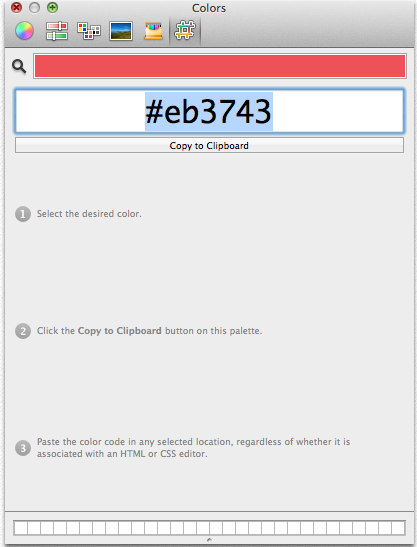
\includegraphics[width=0.4\textwidth]{images/pixelmator.png}}
\end{frame}

\subsection{Основы 2}
\begin{frame}[fragile]
  \frametitle{Где используются системы счисления?}
  \centerline{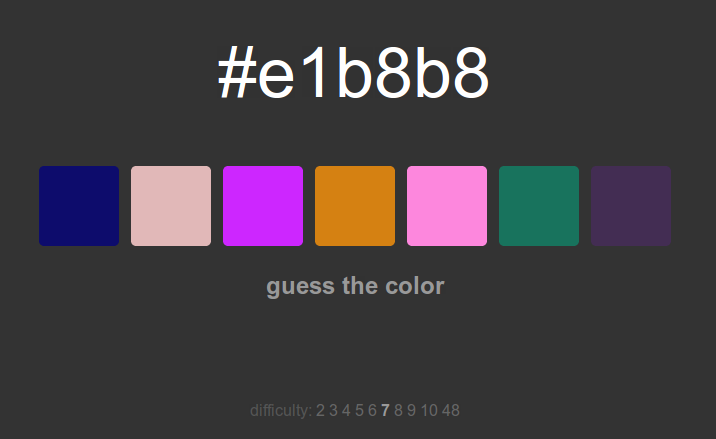
\includegraphics[width=0.9\textwidth]{images/guess-color.png}}
\end{frame}

\subsection{Раз}
\begin{frame}
  \frametitle{Системы счисления}
  \begin{itemize}
    \item Что такое ``системы счисления'' и где они используются?
    \item Система счисления --- это символический способ записи чисел.
    \item Стандартная используемая ныне система счисления --- арабская (индийская).
  \end{itemize}
\end{frame}

\subsection{Основы 2}
\begin{frame}[fragile]
  \frametitle{Арабская система счисления}
  \centerline{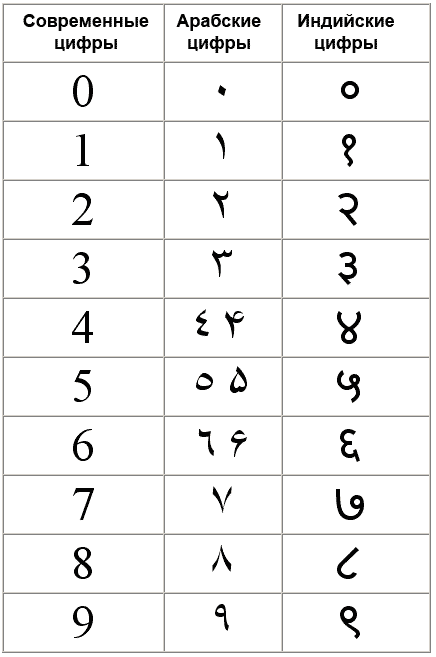
\includegraphics[width=0.4\textwidth]{images/arabian_numbers.png}}
\end{frame}

\subsection{Римская система}
\begin{frame}[fragile]
  \frametitle{Римская система счисления}
  \begin{itemize}
    \item Помимо арабской широко известна \emph{римская система счисления}.
    \item MMXII --- 2012 г. в римской системе.
    \item XCIV --- 94 в римской системе счисления.
    
    \begin{table}
      \begin{tabular}{ccccccc}
      I & V & X & L & C & D & M \\
      1 & 5 & 10 & 50 & 100 & 500 & 1000 \\
      \end{tabular}
    \end{table}
    
    \item \textbf{М}ы \textbf{D}арим \textbf{С}очные \textbf{L}имоны, \textbf{Х}ватит \textbf{V}сем \textbf{I}х.
  \end{itemize}
\end{frame}

\subsection{Задание}
\begin{frame}
  \begin{center}
    \Huge{Задание}
  \end{center}
  \begin{center}
    \Large{Посчитайте и запишите дату (дата, месяц, год) полёта первого человека в космос в римской системе счисления.}
  \end{center}
\end{frame}

\subsection{Позиционные и непозиционные}
\begin{frame}[fragile]
  \frametitle{Позиционные и непозиционные ССч}
  \begin{itemize}
    \item В римской системе счисления практически не важно, в каком порядке записываются символы, так как значение вычисляется в виде суммы всех элементов.
    \item С другой стороны, в арабской системе счисления значение числа строго зависит от его расположения (сравните: 24 и 42).
    \item Системы счисления, в которых значение числа зависит от его расположения, называют \textbf{позиционными}.
    \item Не зависит --- \textbf{непозиционные}.
  \end{itemize}
\end{frame}

\subsection{Майя}
\begin{frame}[fragile]
  \frametitle{Конец близок...}
  \begin{figure}
    \centerline{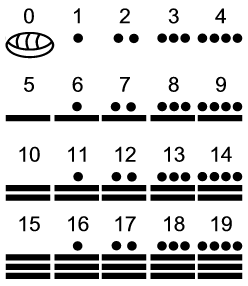
\includegraphics[width=0.4\textwidth]{images/maya.png}}
    \caption{Непозиционная система счисления майя}
  \end{figure}
\end{frame}

\section{Позиционные}
\subsection{Позиционные}
\begin{frame}[fragile]
  \frametitle{Позиционные системы счисления}
  \begin{itemize}
    \item Информатика обычно рассматривает позиционные системы счисления.
    \item Наиболее простым примером является \emph{десятичная система счисления}, которой мы пользуемся в жизни.
    \item Почему она называется десятичной?
    \item Потому что при вычислении значения числа используются его десятичное представление:
    $$
      1237 = 7 + 3\cdot 10 + 2\cdot 100 + 1\cdot 1000
    $$
    $$
      1237 = 7\cdot 10^0 + 3\cdot 10^1 + 2\cdot 10^2 + 1\cdot 10^3
    $$
  \end{itemize}
\end{frame}

\subsection{Другие основания}
\begin{frame}[fragile]
  \frametitle{Основание системы счисления}
  \begin{itemize}
    \item Число 10, являющееся базой для нашей обычной системы счисления, называется \emph{основанием} системы счисления.
    \item Основания могут быть и другими:
  \end{itemize}
  \begin{center}
  \begin{tabular}{cc}
    \hline
    \hline
      Основание & Название \\ 
    \hline
    \hline
      2 & двоичная \\
      3 & троичная \\
      4 & четвертичная \\
      5 & пятеричная \\
      11 & одиннадцатеричная \\
      16 & шестнадцатеричная \\
      .. & ... \\
  \end{tabular}
  \end{center}
\end{frame}

\subsection{Двоичная}
\begin{frame}[fragile]
  \frametitle{Двоичная система счисления}
  \begin{itemize}
    \item Двоичная система счисления состоит из всего из двух цифр: 0 и 1.
    \item То есть, никаких цифр 2, 3 и т.п. в этой системе счисления нет и быть не может.
    \item Но как понять, что число 100 --- это число в двоичной, а не в десятичной системе счисления?
    \item Для этого к числу добавляют специальный индекс, показывающий основание системы счисления:
    $$
      100_2
    $$
    \item Если индекс отсутствует, по умолчанию предполагают, что число находится в десятичной системе счисления.
  \end{itemize}
\end{frame}

\subsection{Таблица оснований}
\begin{frame}[fragile]
  \frametitle{Таблица систем счисления}
  \begin{tabular}{ccc}
    \hline
    \hline
    Основание & Название & Какие цифры входят? \\ 
    \hline
    \hline
    2 & двоичная & 0, 1 \\
    3 & троичная & 0, 1, 2 \\
    4 & четвертичная & 0, 1, 2, 3 \\
    5 & пятиричная & 0, 1, 2, 3, 4 \\
    6 & шестеричная & 0, 1, 2, 3, 4, 5 \\
    7 & семиричная & 0, 1, 2, 3, 4, 5, 6 \\
    8 & восьмиричная & 0, 1, 2, 3, 4, 5, 6, 7 \\
    9 & девятиричная & 0, 1, 2, 3, 4, 5, 6, 7, 8 \\
  \end{tabular}
\end{frame}

\subsection{Задачи}
\begin{frame}
  \begin{itemize}
    \item \Large{В каких системах счисления может быть число $123$?}
    \item \Large{В какой системе счисления число $243_7$}
    \item \Large{В какой системе счисления число $1001$}
  \end{itemize}
\end{frame}

\section{Перевод в десятичную}
\subsection{Перевод}
\begin{frame}
  \begin{center}
    \Huge{Как перевести в десятичную систему из другой?}
  \end{center}
\end{frame}

\subsection{Перевод 2}
\begin{frame}[fragile]
  \frametitle{}
  \begin{itemize}
    \item Для перевода в десятичную систему счисления нужно умножать цифры числа в обратном порядке на последовательные степени основания.
    \item $1011_2 &=& 1\cdot 2^0 + 1\cdot 2^1 + 0\cdot 2^2 + 1\cdot 2^3 = 1 + 2 + 0 + 8 = 11$
    \item $102_3 &=& 2\cdot 3^0 + 0\cdot 3^1 + 1\cdot 3^2 = 2 + 0 + 9 = 11$
    \item $35_9 &=& 5\cdot 9^0 + 3\cdot 9^1 = 5 + 27 = 32$
    \item $100111_2 = $ ?
    \item $1220_3 = $ ?
    \item $551_6 = $ ?
    \item $1234_5 = $ ?
    \item $711_8 = $ ?
  \end{itemize}
\end{frame}

\subsection{Обратно}
\begin{frame}
  \begin{center}
    \Huge{А как перевести обратно?}
  \end{center}
\end{frame}

\subsection{25 в 2}
\begin{frame}[fragile]
  \frametitle{Перевод из десятичной: 25 в двоичную}
  \centerline{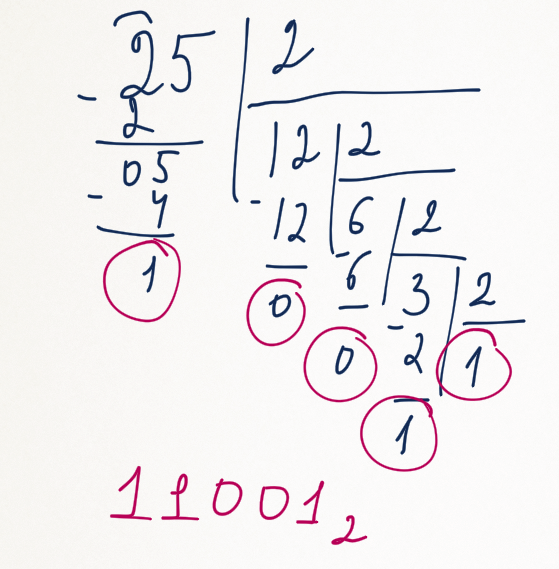
\includegraphics[width=0.6\textwidth]{images/25_2.png}}
\end{frame}

\subsection{35 в 3}
\begin{frame}[fragile]
  \frametitle{Перевод из десятичной: 35 в троичную}
  \centerline{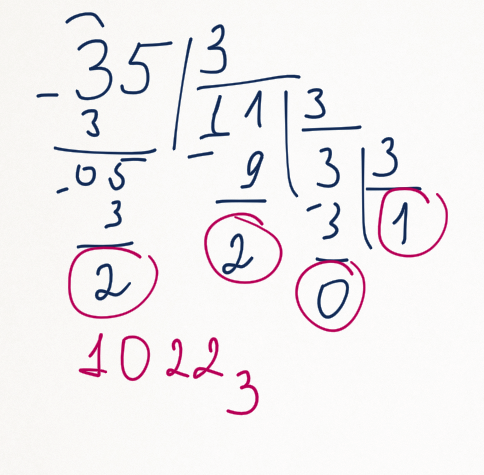
\includegraphics[width=0.6\textwidth]{images/35_3.png}}
\end{frame}

\subsection{Помни}
\begin{frame}
  \begin{center}
    \Huge{Запомнить}
  \end{center}
  \begin{center}
    \Large{Остатки записываем всегда справа налево!}
  \end{center}
\end{frame}

\subsection{Задачи на перевод}
\begin{frame}[fragile]
  \frametitle{Задачи}
  \begin{itemize}
    \item Задача 1. Перевести в четвертичную число $39$.
    \item Задача 2. Перевести в девятиричную число $231$.
    \item Задача 3. Перевести в двоичную число $1024$.
    \item Задача 4. Перевести в двоичную число $512$.
    \item Задача 5. Перевести в семиричную число $3456$.
    \item Задача 6. Перевести в троичную систему счисления число $110010_2$.
    \item Задача 7. Перевести в пятиричную систему счисления число $1202_3$.
  \end{itemize}
\end{frame}

\end{document}